% Talk (10--15 min) on Finzi et al., "From Entropy to Epiplexity", arXiv:2601.03220v2, 16 March 2026 (latest version).
% figs/ holds the vector figures of the arXiv v2 source (byte-identical to v1), unchanged; slides crop them with `trim'.
% Statement and figure numbers ("Thm. 9 of the paper", "Fig. 3") follow v2; v2 kept the v1 numbering.
% Build (twice): pdflatex epiplexity_talk.tex
% Audience questions appear after the main discussion as mini-test material.
\documentclass[aspectratio=169,notheorems]{beamer}
\usetheme{default}
\usefonttheme{professionalfonts}
\setbeamersize{text margin left=8mm,text margin right=8mm}
\setbeamertemplate{navigation symbols}{}
\setbeamertemplate{footline}[frame number]
\setbeamertemplate{itemize item}{--}
\setbeamertemplate{itemize subitem}{--}
\usepackage[T1]{fontenc}
\usepackage{lmodern}
\usepackage{amsmath,amssymb,mathtools,booktabs,array}
\usepackage{microtype}
\usepackage{natbib}
\renewcommand{\bibsection}{}
\definecolor{myblue}{RGB}{25,75,130}
\setbeamercolor{structure}{fg=myblue}
\setbeamercolor{frametitle}{fg=myblue}
\setbeamerfont{frametitle}{size=\large,series=\bfseries}
\setbeamertemplate{blocks}[rounded][shadow=false]
\setbeamercolor{block title}{fg=myblue,bg=myblue!12}
\setbeamercolor{block body}{bg=myblue!4}
\setbeamertemplate{theorems}[numbered]
% one counter per kind; upright bodies
\theoremstyle{definition}
\newtheorem{definition}{Definition}
\newtheorem{theorem}{Theorem}
\newtheorem{proposition}{Proposition}
\newcommand{\E}{\mathbb{E}}
\newcommand{\KL}{\mathrm{KL}}
\newcommand{\MDL}{\mathrm{MDL}}
\newcommand{\Dt}{\mathcal{D}}
\newcommand{\PT}{\mathcal{P}_T}
\newcommand{\Poly}{\mathrm{Poly}}
\newcommand{\prog}{\mathrm{P}}
\DeclareMathOperator*{\argmin}{arg\,min}
% one sentence of provenance under a figure
\newcommand{\src}[1]{{\scriptsize\color{black!60}#1\par}}

\begin{document}
% ============================================================ TITLE
\begin{frame}[plain]
\centering
\vspace*{1.2em}
{\LARGE\bfseries\color{myblue} From Entropy to Epiplexity}\\[0.5em]
{\large Rethinking Information for Computationally Bounded Intelligence}\\[1.8em]
Marc Finzi, Shikai Qiu, Yiding Jiang, Pavel Izmailov, J.~Zico Kolter, Andrew Gordon Wilson\\[0.2em]
{\small Carnegie Mellon University, New York University}\\[0.2em]
{\small arXiv:2601.03220, version~2, 16 March 2026}\\[2.2em]
Speaker: Alexey Kravatskiy
\end{frame}
% ============================================================ PARADOXES
\begin{frame}{Three apparent paradoxes of information}
\small
\begin{block}{1. Deterministic computation cannot increase information}
Yet self-play and synthetic data can improve a model's capabilities.
\end{block}
\begin{block}{2. Total information does not depend on prediction order}
Yet language-model loss can differ between forward and reverse text.
\end{block}
\begin{block}{3. Likelihood modelling targets the data distribution}
Yet prediction can require inference absent from the generating procedure.
\end{block}
\smallskip
\src{Section~5, \citet{finzi2026}. These are apparent tensions, not contradictions of the classical results.}
\end{frame}
% ------------------------------------------------------------
\begin{frame}{Shannon entropy and Kolmogorov complexity}
\small
\begin{columns}[T]
\begin{column}{0.47\textwidth}
\textbf{Shannon entropy: a distribution}
\[
\begin{aligned}
p(x)&=\Pr(X=x),\\[-0.15em]
H(X)&=\E[-\log_2 p(X)].
\end{aligned}
\]
For discrete $X$, entropy is a lower bound on the expected length of any binary prefix code.

\medskip
Uniform $n$-bit strings: $H(X)=n$.

\smallskip
A fixed string: $H(X)=0$.
\end{column}
\begin{column}{0.47\textwidth}
\textbf{Kolmogorov complexity: a string}
\[
K(x)=\min_{p:\,\mathcal U(p)=x}|p|.
\]
The shortest self-delimiting program that outputs $x$ and halts on a fixed prefix-free universal Turing machine $\mathcal U$.

\medskip
An alternating string is specified by its rule and length. Most uniform $n$-bit strings require at least $n-O(1)$ program bits.
\end{column}
\end{columns}
\medskip
\src{$K(x)$ is uncomputable in general. Definition~1 and Section~2.1, \citet{finzi2026}.}
\end{frame}
% ------------------------------------------------------------
\begin{frame}{Paradox 1: deterministic computation and new information}
\small
For discrete $X$ and a fixed computable transformation $f$,
\[
H(f(X))\le H(X),\qquad K(f(x))\le K(x)+K(f)+c.
\]
The output has a description: specify the input and the program for $f$, then run it. These bounds do not restrict how long that computation takes.

\begin{block}{Example: expanding a random seed}
A pseudorandom generator transforms $k$ seed bits into $n>k$ output bits. The output still has entropy at most $k$ and a description of length at most $k+K(G)+O(\log_2 k)$. For a secure generator, no randomized test with runtime polynomial in $k$ distinguishes the output from uniform data with non-negligible advantage.
\end{block}
AlphaZero learns a policy and a value function through self-play. Specifying its algorithm and random seed can take far fewer bits than storing the trained network, but reconstructing that network requires running the training procedure.

\medskip
\src{Negligible advantage: eventually smaller than $k^{-m}$ for every fixed $m>0$. Section~5.1 and Theorem~12, \citet{finzi2026}; the theorem uses polynomial-length advice independent of the sampled seed.}
\end{frame}
% ------------------------------------------------------------
\begin{frame}{Paradox 2: equal information, different prediction costs}
\small
The chain rule gives the same joint entropy in either order:
\[
H(X)+H(Y\mid X)=H(X,Y)=H(Y)+H(X\mid Y).
\]
Each order describes the same pair. The identity does not bound the cost of evaluating or sampling from the conditional distributions.

\begin{block}{Example: a bijection computable in polynomial time}
Let $X$ be uniform on $n$-bit strings and $Y=f(X)$. Since $f$ is a bijection, $Y$ is also uniform and both conditional entropies are zero.
\begin{itemize}\setlength{\itemsep}{0.4em}
\item \textbf{Input first:} encode $X$ in $n$ bits, then compute $Y=f(X)$.
\item \textbf{Output first:} encode $Y$ in $n$ bits, then recover $X=f^{-1}(Y)$.
\end{itemize}
One-wayness means that no randomized algorithm with runtime polynomial in $n$ recovers $X$ from $f(X)$ with non-negligible probability over uniform $X$.
\end{block}
Prediction order can therefore affect what a model can compute. The paper studies this with cellular-automaton pairs and reordered chess data.

\smallskip
\src{Section~5.2 and Theorem~13, \citet{finzi2026}. The theorem also allows polynomial-length advice independent of the sampled input; one-wayness is an assumption.}
\end{frame}
% ------------------------------------------------------------
\begin{frame}{Paradox 3: can prediction require more than generation?}
\small
Likelihood training minimizes
\[
L_Q(P)=\E_{Y\sim Q}[-\log_2 P(Y)].
\]
When the model class contains the data distribution $Q$, the minimum is attained at $P=Q$.

\medskip
Does matching the distribution require only reproducing the generator's computations? Consider a mystery story:

\begin{columns}[T]
\begin{column}{0.47\textwidth}
\begin{block}{The author generates the story}
Choose the culprit, then write consistent clues. The culprit is already known.
\end{block}
\end{column}
\begin{column}{0.47\textwidth}
\begin{block}{The model predicts the reveal}
Given only the clues, assign probabilities to possible culprits before the reveal.
\end{block}
\end{column}
\end{columns}
\medskip
Prediction requires inference from clues to culprit; generation does not. The paper calls this \textbf{induction}: inference about unobserved variables. Under a time bound, it may require a different algorithm from the generator's.
\par\smallskip
\src{Section~5.3 and the mystery-story example in Section~5.3.1, \citet{finzi2026}.}
\end{frame}
% ============================================================ FORMAL PROBLEM STATEMENT
\begin{frame}{Time-bounded probabilistic models}
\small
Fix a prefix-free universal Turing machine. A program $\prog$ implements the same distribution $P$ in two modes: evaluate $P(x)$ or sample $x\sim P$. Each call must finish within $T(n)$ steps, for every input.

\begin{block}{Example: one autoregressive model, fixed parameters $\theta$}
The network outputs conditional probabilities $p_\theta(x_j\mid x_{<j})$.
\begin{itemize}\setlength{\itemsep}{0.5em}
\item \textbf{Evaluation:} supply the observed prefixes and multiply:
\[
P_\theta(x)=\prod_{j=1}^{n}p_\theta(x_j\mid x_{<j}).
\]
\item \textbf{Sampling:} draw $x_1$, then $x_2\mid x_1$, and so on, using the same conditionals and fresh random bits.
\end{itemize}
\end{block}
$\PT$ is the set of programs satisfying both runtime bounds and whose sampler agrees with the evaluated probabilities. $|\prog|$ is the program length in bits.
\par\smallskip
\src{Definition~7, \citet{finzi2026}: $T$ is non-decreasing and time-constructible; probabilities are exact, normalized and have finite binary expansions.}
\end{frame}
% ------------------------------------------------------------
\begin{frame}{Epiplexity: the two-part description}
\small
For $X$ on $\{0,1\}^n$, choose an admissible model minimizing the expected two-part description length:
\[
\prog^\star\in\argmin_{\prog\in\PT}
\bigl\{|\prog|+\E[-\log_2 P(X)]\bigr\}.
\]
Among minimizers, select one with the shortest program.

\begin{columns}[T]
\begin{column}{0.47\textwidth}
\begin{block}{Epiplexity: model description}
\[
S_T(X):=|\prog^\star|.
\]
Length of the selected model's program.
\end{block}
\end{column}
\begin{column}{0.47\textwidth}
\begin{block}{Time-bounded entropy: data description}
\[
H_T(X):=\E[-\log_2 P^\star(X)].
\]
Expected data-code length using that model.
\end{block}
\end{column}
\end{columns}
\[
\MDL_T(X)=S_T(X)+H_T(X).
\]
\src{Definition~8, \citet{finzi2026}.}
\end{frame}
% ------------------------------------------------------------
\begin{frame}{Examples: random bits and a repeated pattern}
\small
Assume the length $n$ is specified and the time bound permits the models below.

\begin{block}{Uniform bits: $X\sim U_n$}
A constant-length program assigns $P(x)=2^{-n}$ to every $n$-bit string, so
\[
\MDL_T(X)\le n+c.
\]
If some $P(x)=0$, the loss is infinite. Otherwise $\prod_xP(x)\le(2^{-n})^{2^n}$; taking $-\log_2$ and dividing by $2^n$ gives
\[
\mathbb E_{U_n}[-\log_2P(U_n)]\ge n.
\]
Hence $n\le H_T(X)\le n+c$ and $S_T(X)\le c$.
\end{block}

\begin{block}{Alternating strings: two equally likely outcomes}
$X=0101\ldots$ or $1010\ldots$, each with probability $\tfrac12$.
A constant-length program generates either pattern in linear time.
\[
S_T(X)=O(1),\qquad H_T(X)=O(1).
\]
\end{block}
\end{frame}
% ============================================================ THEORY
\begin{frame}{Cryptographic consequences of the time bound}
\small
\begin{itemize}\setlength{\itemsep}{0.65em}
\item \textbf{Pseudorandom generator.} $G$ maps $k$ random seed bits to $n>k$ output bits.
      $H(G(U_k))\le k$, yet for a secure generator $H_{\Poly}(G(U_k))\approx n$ and $S_{\Poly}(G(U_k))=O(1)$.
\item \textbf{One-way function.} Computing $f(x)$ takes polynomial time. No randomized polynomial-time algorithm finds a preimage with non-negligible probability over uniformly sampled inputs.
      For a one-way \emph{permutation}, the paper proves that the two factorization orders have different time-bounded entropies.
\end{itemize}

\medskip
\src{Theorems~9 and~13, \citet{finzi2026}. These results assume security against non-uniform probabilistic polynomial-time algorithms.}
\end{frame}
% ------------------------------------------------------------
\begin{frame}{Conditional epiplexity: predicting labels from inputs}
\small
For supervised data $(X,Y)$, the decoder already has the input $X$.
The model evaluates $P(y\mid x)$ and samples $Y\mid X=x$ within the bound for each fixed $x$.

\[
\prog^\star_{Y\mid X}\in\argmin_{\prog\in\mathcal P_T^X}
\left\{|\prog|+\E_{X,Y}[-\log_2 P(Y\mid X)]\right\}.
\]
\[
S_T(Y\mid X):=|\prog^\star_{Y\mid X}|,\qquad
H_T(Y\mid X):=\E_{X,Y}[-\log_2 P^\star(Y\mid X)].
\]
\begin{block}{Example: image classification}
The model code describes the classifier. The data code describes the labels given the images; it does not encode the images.
\end{block}
In general,
$H_T(Y\mid X)\ne H_T(X,Y)-H_T(X)$.

\medskip
\src{Definition~11, \citet{finzi2026}.}
\end{frame}
% ============================================================ METHOD
\begin{frame}{Compute budget for training and evaluation}
\small
The experiments restrict the search to models trained with a chosen architecture and optimiser. To decode the empirical two-part code, first reconstruct the weights by replaying training, then evaluate the target data with those weights. Let $N$ count parameters, $D$ training tokens and $\Dt$ evaluation tokens.
\[
\underbrace{6ND}_{\text{replay training: }2ND+4ND}
+\underbrace{2N\Dt}_{\text{evaluation: forward only}}\le T.
\]
\begin{itemize}\setlength{\itemsep}{0.6em}
\item A dense forward pass costs roughly $2N$ FLOPs per token: one multiplication and one addition per parameter.
\item Backpropagation computes gradients for activations and weights: roughly $4N$ FLOPs per token, twice the forward pass.
\end{itemize}
The terms add because the decoder performs these stages in sequence. Sampling does not involve training; after the weights are reconstructed, it is a separate call that must satisfy its own sampling bound.
For each $(N,D)$ satisfying the budget, estimate the model-code length and add the validation loss (bits per token) multiplied by $\Dt$. Retain the run with the smallest sum.
\par\medskip
\src{Sections~3--4 and Appendix~B.1, \citet{finzi2026}. This is empirical compute accounting. Formal membership in $\PT$ requires both evaluation and sampling to satisfy the bound separately.}
\end{frame}
% ------------------------------------------------------------
\begin{frame}{Prequential coding: transmit data and reproduce training}
\small
Both sides share the initial training state $\theta_0$ (weights and optimiser state), update rule $A$, schedule and random seed. Let $Z_i$ be the next training batch and $P_i=P_{\theta_i}$ the model before its update.
\begin{enumerate}\setlength{\itemsep}{0.6em}
\item \textbf{Encoder:} arithmetic-code $Z_i$ under $P_i$; transmit the resulting bits.
\item \textbf{Decoder:} use its identical $P_i$ and those bits to recover exactly $Z_i$.
\item \textbf{Both:} compute $\theta_{i+1}=A(\theta_i,Z_i)$, then repeat.
\end{enumerate}
\[
L_{\mathrm{preq}}=\sum_{i=0}^{M-1}-\log_2 P_i(Z_i).
\]
The message reconstructs the exact training batches \emph{and} the final state $\theta_M$.
\par\medskip
\src{Ideal lengths omit arithmetic-coding and setup overhead. Prequential approach: \href{https://doi.org/10.2307/2981683}{Dawid (1984)}; neural-network coding: \href{https://arxiv.org/abs/1802.07044}{Blier and Ollivier (2018)}.}
\end{frame}
% ------------------------------------------------------------
\begin{frame}{Estimating model bits from the training-loss curve}
\small
Let $Z=(Z_0,\ldots,Z_{M-1})$. The prequential message reconstructs $(Z,P_M)$; given $P_M$, the data alone have a code of length $L_{\mathrm{final}}$.

\medskip
\begin{columns}[c]
\begin{column}{0.60\textwidth}
The unbounded algorithmic chain rule suggests
\[
K(Z,P_M)\approx K(P_M)+K(Z\mid P_M).
\]
Substituting the two code lengths gives
\[
\begin{aligned}
L_{\mathrm{final}}&=\sum_{i=0}^{M-1}-\log_2 P_M(Z_i),\\
\widehat K_{\mathrm{preq}}&=L_{\mathrm{preq}}-L_{\mathrm{final}}.
\end{aligned}
\]
This is a \textbf{heuristic}: subtracting two upper bounds need not bound $K(P_M)$, and the chain rule gives no decoder within $T$.
\end{column}
\begin{column}{0.36\textwidth}
\centering
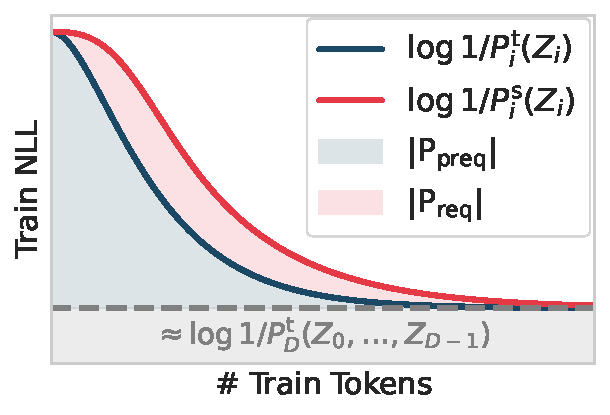
\includegraphics[width=\linewidth]{figs/requential_illustration.pdf}
\end{column}
\end{columns}
\par\smallskip
\src{Section~4.1 and Fig.~2a, \citet{finzi2026}. The unbounded algorithmic chain rule has logarithmic overhead in this form; it does not give a time-bounded identity.}
\end{frame}
% ------------------------------------------------------------
\begin{frame}{Requential coding: reconstruct a model from sample indices}
\small
At step $i$, the encoder has a teacher checkpoint $Q_i$, typically trained on real data. Both sides share a student $P_i=P_{\theta_i}$, initial state, update rule $A$ and random seed $s$.
\begin{enumerate}\setlength{\itemsep}{0.45em}
\item Generate indexed proposals $Y_i^{(j)}\sim P_i$, reproducible from $(s,i,j)$.
\item The encoder uses \href{https://proceedings.mlr.press/v162/theis22a.html}{\textbf{relative entropy coding}} to select $J_i$ so that $\widetilde Z_i=Y_i^{(J_i)}\sim Q_i$, then sends a prefix code for $J_i$.
\item The decoder regenerates $\widetilde Z_i$. Both update $\theta_{i+1}=A(\theta_i,\widetilde Z_i)$; repeating reconstructs the final student.
\end{enumerate}
If $Q_i=P_i$, the first proposal suffices; its random bits need no transmission.
\[
\begin{aligned}
d_i&:=\KL(Q_i\Vert P_i)=\E_{Z\sim Q_i}\!\left[\log_2\frac{Q_i(Z)}{P_i(Z)}\right],\\
\E[\ell_i\mid\text{history}]&\le d_i+2\log_2(1+d_i)+\kappa,\qquad\kappa<5.21.
\end{aligned}
\]
Here $\ell_i$ is the index-message length. The leading model-length estimate is $\widehat K_{\mathrm{req}}=\sum_i d_i$.
\par\smallskip
\src{Relative entropy coding: \href{https://proceedings.mlr.press/v162/theis22a.html}{Theis and Ahmed (ICML, 2022)}. Protocol and bound: \citet{qiu2026}, Section~3.1 and Appendix~A.1. Assume $P_i(z)>0$ whenever $Q_i(z)>0$; setup and logarithmic overhead are omitted from the leading estimate.}
\end{frame}
% ============================================================ EXPERIMENTS
\begin{frame}{Cellular automata: simple dynamics, different model parts}
\small
An \emph{elementary cellular automaton} (ECA) updates binary cells in parallel from their three-cell neighbourhoods \citep{wolfram2002}.\par
\textbf{Setting.} $64$ periodic cells; $Y=F_r^{48}(X)$; transformer sweep; requential code.

\smallskip
\begin{columns}[T]
\begin{column}{0.47\textwidth}
\centering
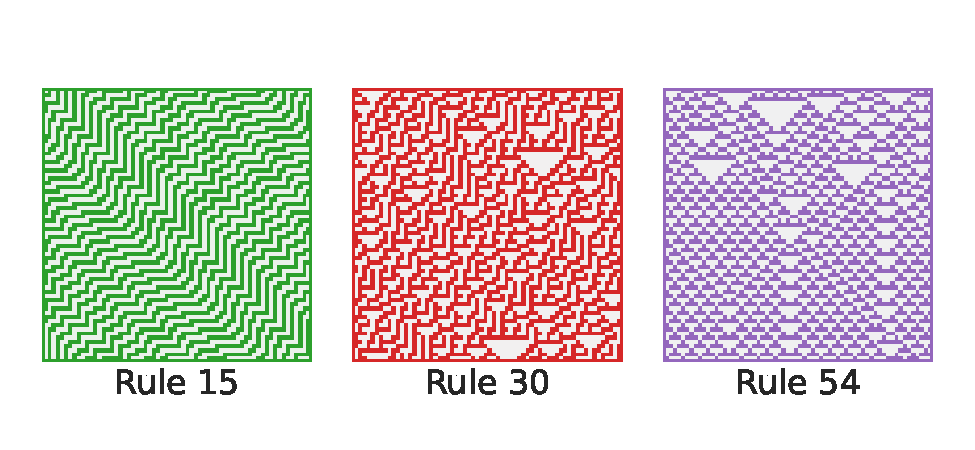
\includegraphics[width=0.72\linewidth,trim=18 19 15 38,clip]{figs/eca_spacetime.pdf}

\smallskip
\begin{tabular}{@{}lccc@{}}
\toprule
Rule & 15 & 30 & 54 \\
\midrule
$S_T(Y\mid X)$, bits & $2\times10^5$ & $\approx0$ & $5.4\times10^6$ \\
$H_T(Y\mid X)$, bits & $\approx0$ & $10^8$ & $1.5\times10^7$ \\
\bottomrule
\end{tabular}
\end{column}
\begin{column}{0.45\textwidth}
\centering
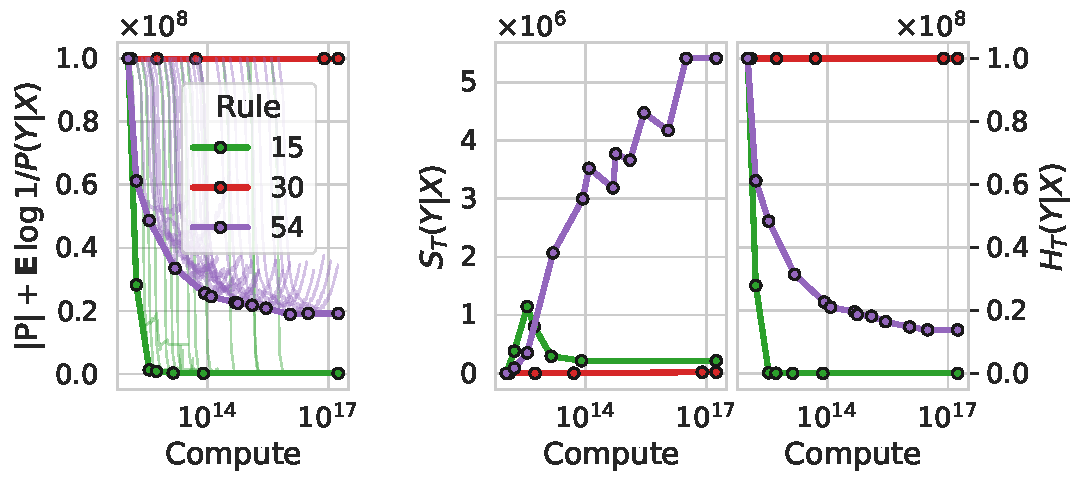
\includegraphics[height=3.6cm,trim=180 0 0 0,clip]{figs/eca_rules_measurements.pdf}
\end{column}
\end{columns}
\src{Left: rollouts, time downward. Right: $S_T$ and $H_T$ against compute in FLOPs. Table: our estimates from the plots at $10^{17}$ FLOPs. Source: Fig.~3 of \citet{finzi2026}.}
\end{frame}
% ------------------------------------------------------------
\begin{frame}{Epiplexity need not increase with compute}
\begin{columns}[T]
\begin{column}{0.52\textwidth}
\small
\textbf{Setting.} ECA rule~54, $64$ updates. The non-looped model predicts the final state; the looped model also predicts intermediate states.

\medskip
\begin{itemize}\setlength{\itemsep}{0.2em}
\item Below $10^{15}$ FLOPs, the non-looped model gives the shorter estimated code; its model part reaches $1.45\times10^7$ bits.
\item Above that budget, the looped model gives the shorter code. Repeated application of the simple dynamics becomes preferable.
\item The authors interpret this as emergence: limited compute favours prediction from large-scale patterns.
\end{itemize}
\end{column}
\begin{column}{0.44\textwidth}
\centering
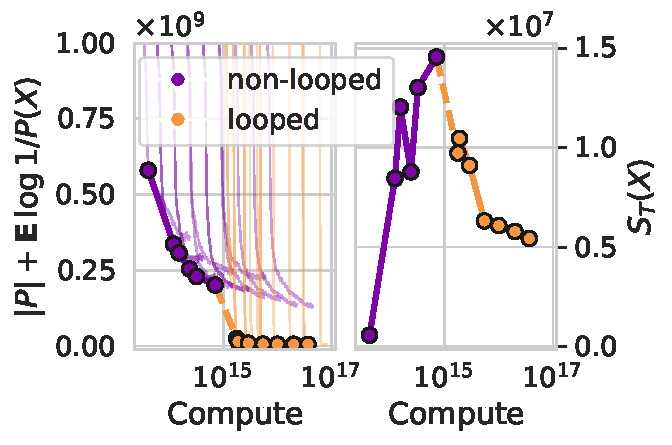
\includegraphics[width=\linewidth]{figs/eca_emergence.pdf}
\raggedright
\src{Two-part code and $S_T$ against compute in FLOPs. Source: Fig.~6 of \citet{finzi2026}.}
\end{column}
\end{columns}
\end{frame}
% ------------------------------------------------------------
\begin{frame}{Paradox 3 in the experiment: hidden inputs}
\small
\textbf{Generate data:} start with a uniformly random row $Z$ of $32$ binary cells on a ring.
\begin{itemize}\setlength{\itemsep}{0.2em}
\item $m_h$ deletes the first $h$ cells ($h=0,\ldots,5$); the observed input is $X=m_h(Z)$.
\item $f$ applies rule~30 to the \emph{complete} row four times; the target is $Y=f(Z)$.
\end{itemize}

\smallskip
\begin{columns}[c]
\begin{column}{0.4\textwidth}
\centering
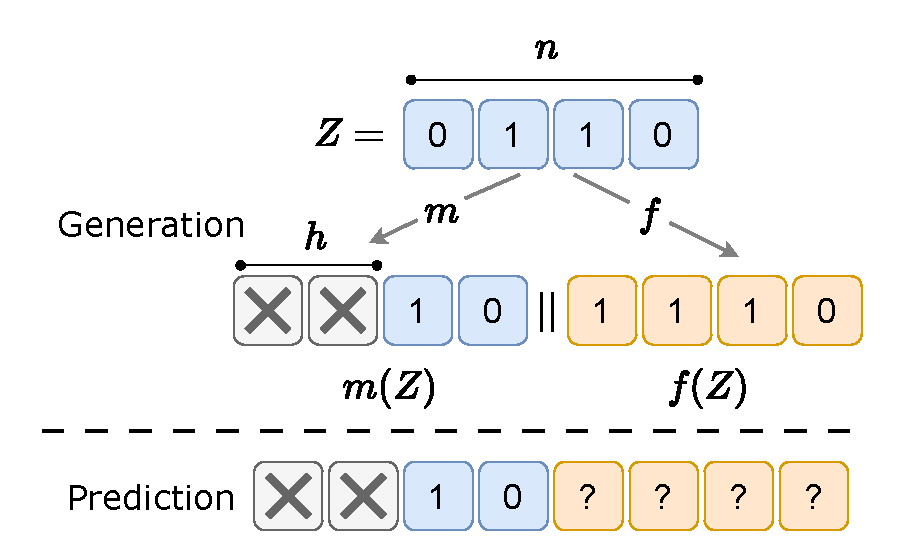
\includegraphics[height=2.6cm]{figs/hidden_bits_illustration.pdf}
\end{column}
\begin{column}{0.5\textwidth}
\centering
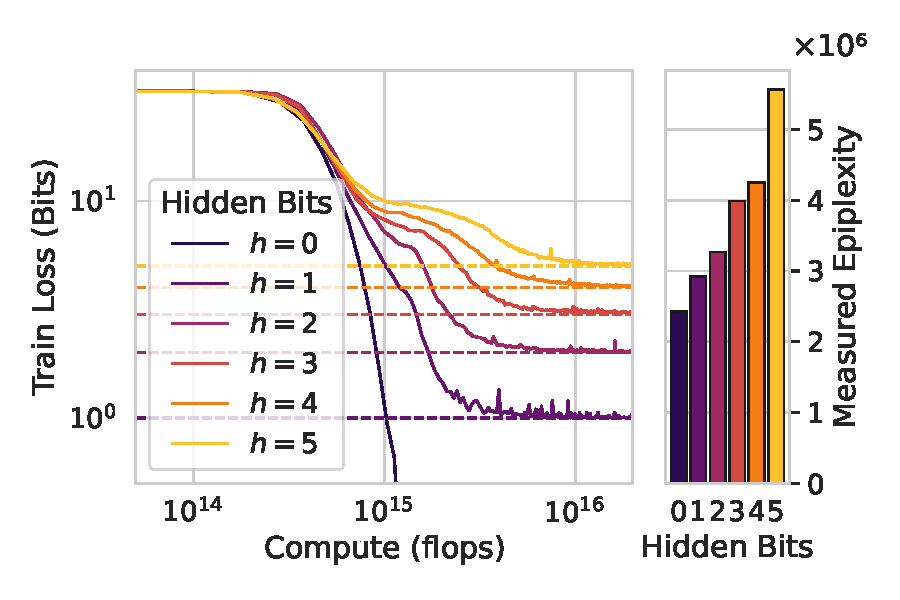
\includegraphics[height=3.1cm]{figs/induction_hard.pdf}
\end{column}
\end{columns}
\src{Fig.~5b, \citet{finzi2026}: prediction loss against compute (dashed: reported $h$-bit baseline), and estimated $S_T$.}
\begin{itemize}\setlength{\itemsep}{0.3em}
\item A transformer predicts $Y$ given $X$; requential coding estimates its model part. With $h$ hidden cells, $2^h$ complete initial rows are consistent with $X$.
\item More hidden cells require more training compute to reach the baseline and increase the model-part estimate: evidence of inference absent from the generator.
\end{itemize}
\par\smallskip
\src{Section~5.3.1. The plots do not identify the learned algorithm or establish a complexity lower bound.}
\end{frame}
% ------------------------------------------------------------
\begin{frame}{Experiment: the order of chess data}
\small
\textbf{Setting.} Lichess games in two orders: moves $\to$ final board, or board $\to$ moves. Transformer sweep with requential coding.

\smallskip
\begin{columns}[c]
\begin{column}{0.44\textwidth}
\centering
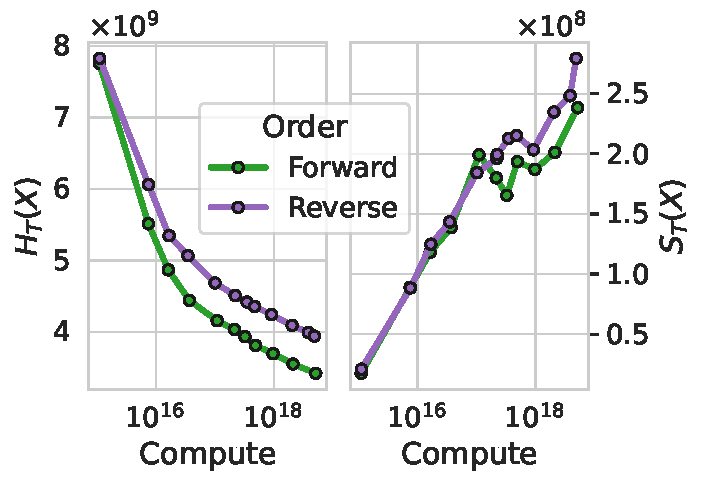
\includegraphics[height=3.0cm]{figs/chess_entropy_and_epi.pdf}
\end{column}
\begin{column}{0.4\textwidth}
\centering
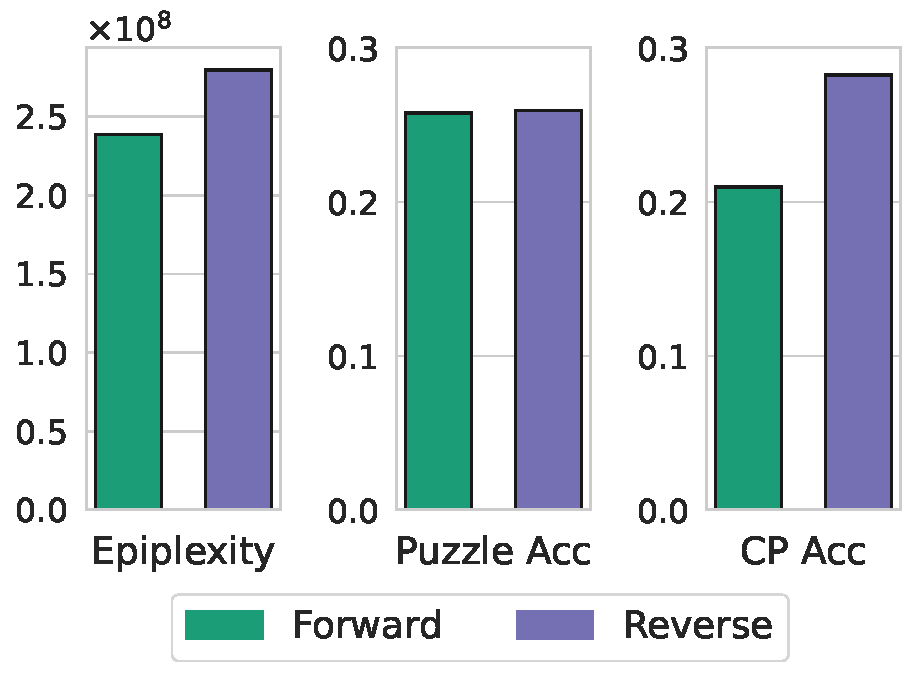
\includegraphics[height=3.0cm]{figs/chess_metrics_bar.pdf}
\end{column}
\end{columns}
\src{Left: $H_T$ and $S_T$ against compute in FLOPs. Right: $S_T$ and accuracy after fine-tuning. Source: Figs.~4c and~7 of \citet{finzi2026}.}
\begin{itemize}
\item At large compute, reverse order gives higher $H_T$ and $S_T$.
\item After fine-tuning, reverse-order models reach $0.28$ board-evaluation accuracy versus $0.21$ for forward-order models; puzzle accuracy is similar.
\end{itemize}
\end{frame}
% ------------------------------------------------------------
\begin{frame}{Application: structure in natural data}
\small
\textbf{Setting.} Equal token budgets and a shared compute bound. Compare OpenWebText, chess and CIFAR-5M with the requential code.

\smallskip
\begin{columns}[T]
\begin{column}{0.38\textwidth}
\centering
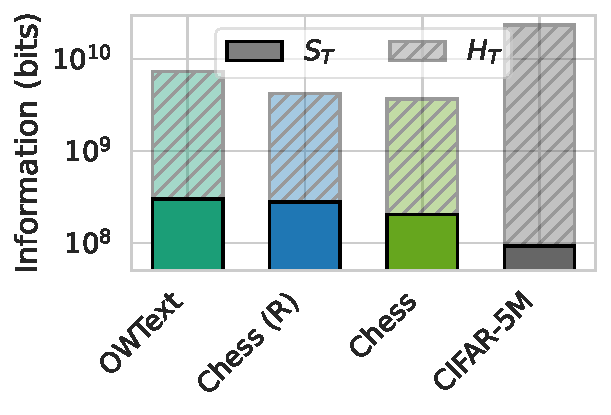
\includegraphics[height=3.3cm]{figs/natural_epi_stacked.pdf}\par
\raggedright
\src{Chess (R): reverse order. Source: Fig.~8a of \citet{finzi2026}. Table: our estimates from the figure.}
\end{column}
\begin{column}{0.58\textwidth}
\begin{tabular}{@{}lccc@{}}
\toprule
Dataset & $S_T$, bits & $\MDL_T$, bits & $S_T/\MDL_T$ \\
\midrule
OpenWebText & $3\times10^8$ & $7\times10^9$ & $4\%$ \\
Chess, reverse & $2.8\times10^8$ & $4\times10^9$ & $7\%$ \\
Chess, forward & $2\times10^8$ & $3.5\times10^9$ & $6\%$ \\
CIFAR-5M & $9\times10^7$ & $2.3\times10^{10}$ & $0.4\%$ \\
\bottomrule
\end{tabular}

\smallskip
\begin{itemize}\setlength{\itemsep}{0.2em}
\item The datasets use the same evaluation-token count and compute bound. Images are encoded as pixel tokens; chess and text use their respective tokenisations.
\item The estimates depend on the tokenisation, model family and compute budget.
\end{itemize}
\end{column}
\end{columns}
\end{frame}
% ============================================================ SUMMARY
\begin{frame}{Conclusions and limitations}
\textbf{Summary}
\begin{itemize}\setlength{\itemsep}{0.3em}
\item $S_T$ counts selected model bits; $H_T$ is the expected data-code length.
\item Computational restrictions can change both the total description length and its decomposition.
\item Epiplexity can be unbounded: some families satisfy $S_{\Poly}(X_n)=\Omega(\log_2 n)$ under one-way-function assumptions.
\item Neural-network estimates combine a model-code estimate with validation loss, optimized under a compute budget.
\end{itemize}
\medskip
\textbf{Limitations}
\begin{itemize}\setlength{\itemsep}{0.3em}
\item $S_T$ is not a guarantee of downstream usefulness.
\item Estimates depend on architecture, optimiser, $T$ and dataset size.
\end{itemize}
\end{frame}
% ============================================================ FOLLOW-UP WORK
\begin{frame}{Follow-up work from Wilson's group}
\small
\begin{block}{Qiu et al. (2026): \href{https://arxiv.org/abs/2607.11883}{\textbf{Requential Coding}}}
A teacher selects examples drawn from the student's predictive distribution. Recording the selection indices reconstructs the student's training trajectory; the coding cost depends on teacher--student disagreement. This yields PAC--Bayes generalization bounds for billion-parameter language models. At fixed loss, larger models can have shorter codes.
\end{block}
\begin{block}{Su et al. (2026): \href{https://arxiv.org/abs/2608.11746}{\textbf{EpiSelect and EpiGen}}}
\textbf{EpiSelect} fits cross-domain loss-scaling laws and adjusts sampling weights to maximize predicted gains in an online epiplexity proxy. \textbf{EpiGen} trains a synthetic-data generator with a policy-gradient reward: the reduction in learner loss on earlier samples after training on a new batch. Both methods report improved downstream performance.
\end{block}
\end{frame}
% ============================================================ LITERATURE
\begin{frame}[t]{Literature: epiplexity and follow-up work}
\begin{thebibliography}{6}\setlength{\itemsep}{0.55em}
\normalsize
\bibitem[Finzi et al.(2026)]{finzi2026}
Marc Finzi, Shikai Qiu, Yiding Jiang, Pavel Izmailov, J.~Zico Kolter, Andrew Gordon Wilson (2026).\\
\href{https://arxiv.org/abs/2601.03220v2}{\color{myblue}\textbf{From Entropy to Epiplexity}}.
\bibitem[Qiu et al.(2026)]{qiu2026}
Shikai Qiu, Marc Finzi, Yujia Zheng, Kun Zhang, Andrew Gordon Wilson (2026).\\
\href{https://arxiv.org/abs/2607.11883}{\color{myblue}\textbf{Requential Coding}}.
\bibitem[Su et al.(2026)]{su2026}
Ellen Su, Andres Potapczynski, Shikai Qiu, Edward Hughes, Andrew Gordon Wilson (2026).\\
\href{https://arxiv.org/abs/2608.11746}{\color{myblue}\textbf{Epiplexity Guided Data Selection and Generation for Out-of-Distribution Generalization}}.
\end{thebibliography}
\end{frame}
\begin{frame}[t]{Literature: background}
\begin{thebibliography}{6}\setlength{\itemsep}{0.7em}
\normalsize
\bibitem[Li and Vit\'anyi(2008)]{livitanyi2008}
Ming Li and Paul Vit\'anyi (2008).\\
\href{https://doi.org/10.1007/978-0-387-49820-1}{\color{myblue}\textbf{An Introduction to Kolmogorov Complexity and Its Applications}}.
\bibitem[Wolfram(2002)]{wolfram2002}
Stephen Wolfram (2002).\\
\href{https://www.wolframscience.com/nks/}{\color{myblue}\textbf{A New Kind of Science}}.
\bibitem[Jiang et al.(2025)]{jiang2025}
Yiding Jiang, Allan Zhou, Zhili Feng, Sadhika Malladi, J.~Zico Kolter (ICLR, 2025).\\
\href{https://arxiv.org/abs/2410.11820}{\color{myblue}\textbf{Adaptive Data Optimization: Dynamic Sample Selection with Scaling Laws}}.
\end{thebibliography}
\end{frame}
\begin{frame}[t]{Literature: sequential and relative entropy coding}
\begin{thebibliography}{6}\setlength{\itemsep}{0.7em}
\normalsize
\bibitem[Dawid(1984)]{dawid1984}
A.~Philip Dawid (1984).\\
\href{https://doi.org/10.2307/2981683}{\color{myblue}\textbf{Present Position and Potential Developments: Some Personal Views. Statistical Theory: The Prequential Approach}}.
\bibitem[Blier and Ollivier(2018)]{blier2018}
L\'eonard Blier and Yann Ollivier (NeurIPS, 2018).\\
\href{https://arxiv.org/abs/1802.07044}{\color{myblue}\textbf{The Description Length of Deep Learning Models}}.
\bibitem[Theis and Ahmed(2022)]{theis2022}
Lucas Theis and Noureldin Y.~Ahmed (ICML, 2022).\\
\href{https://proceedings.mlr.press/v162/theis22a.html}{\color{myblue}\textbf{Algorithms for the Communication of Samples}}.
\end{thebibliography}
\end{frame}
% ============================================================ QUESTIONS
\begin{frame}{Questions for the audience}
\small
\begin{enumerate}\setlength{\itemsep}{0.7em}
\item Let $X\sim U_n$. Which quantity is close to $n$: $S_T(X)$ or $H_T(X)$?
\item In the prequential estimate, which part of the training-loss curve approximates the epiplexity?
\item If $P=Q$, must the model use the same algorithm as the generator?
\end{enumerate}
\end{frame}
% ============================================================ BACKUP
\begin{frame}{Backup: selecting a proposal by rejection sampling}
\small
At one step, let $P$ be the student and $Q$ the teacher. Choose $B\ge\max_z Q(z)/P(z)$, with $P(z)>0$ whenever $Q(z)>0$.
\begin{enumerate}\setlength{\itemsep}{0.5em}
\item The shared seed generates indexed proposals $Y^{(j)}\sim P$ and independent $U_j\sim\mathrm{Uniform}[0,1]$.
\item The encoder accepts the first index $J$ satisfying
\[
U_J\le\frac{Q(Y^{(J)})}{B\,P(Y^{(J)})}.
\]
\item Transmit $J$; the decoder regenerates $Y^{(J)}$ without knowing $Q$.
\end{enumerate}
For a proposal, $\Pr(Y=z,\text{ accept})=P(z)\,Q(z)/(BP(z))=Q(z)/B$. Conditioning on acceptance therefore gives distribution $Q$.

\medskip
More sophisticated REC constructions provide the KL-based length bound on the main slide.
\par\smallskip
\src{\citet{qiu2026}, Fig.~2 and Section~2; \href{https://proceedings.mlr.press/v162/theis22a.html}{Theis and Ahmed (2022)}. Simple rejection sampling can have a much larger coding cost.}
\end{frame}
\begin{frame}{Backup: basic properties}
\begin{proposition}[Sec.~3 of the paper]
Let $c_1,c_2$ be constants independent of $X$. For a random variable $X$ on $\{0,1\}^n$:
\begin{enumerate}
\item $S_T(X)\ge0$ and $H_T(X)\ge0$;
\item $H(X)\le\MDL_T(X)\le n+c_1$;
\item $\MDL_{T'}(X)\le\MDL_T(X)$ whenever $T'(n)\ge T(n)$;
\item $\MDL_{T'}(f^{-1}(X))\le\MDL_T(X)+|\mathrm f|+c_2$ with $T'(n)=T(n)+\mathrm{Time}(\mathrm f)$, for a program $\mathrm f$ that computes a bijection $f$ in fixed time.
\end{enumerate}
\end{proposition}
Property~4 is the analogue of $K(f(x))\le K(x)+K(f)+c$. Under a time bound a short program for $f^{-1}$ gives no short program for $f$.
\begin{theorem}[Thm.~10 of the paper]
If one-way functions secure against probabilistic polynomial-time algorithms with polynomial advice exist, then some random variables $X_n$ on $\{0,1\}^n$ have $S_{\Poly}(X_n)=\Omega(\log_2 n)$.
\end{theorem}
\end{frame}
% ------------------------------------------------------------

\end{document}
